\chapter{概率与统计 - 频率派\&贝叶斯派}
\begin{figure}[ht]
  \centering
  
\includegraphics[width=1\linewidth]{asset/茶桁的AI秘籍_Math_19.png}
\end{figure}

\newpage

本节课, 咱们开始学习「概率\&统计」的部分, 说实话, 这个部分是我觉得最有意思的地方. 

在之前的课程中, 除了导论课给大家过了一遍通识性的各个领域的一些知识之外, 我们已经上过了关于微积分、还有关于先行代数的一些东西. 都是和我们在未来人工智能这个领域所运用到的方面有很强的一个联系, 包括现在我们要学习的概率统计也是一样. 

虽然它是和导论课里面有一点重合, 但是它是一个基础性的东西, 绕不过去. 所以也就给大家简单的回过头来再看一下. 

\section{频数和频率}

这节课, 我们先说一下从一个频数和频率去看待这个概率. 

为什么我们遇到一些决定不了的事情的时候很多人会选择去抛硬币呢?比如说正面朝上代表着去做某一个决定, 反面朝上就表示维持现状. 那为什么人会倾向于用这个抛硬币的方式去决定选择呢?

\begin{figure}[ht]
  \centering
  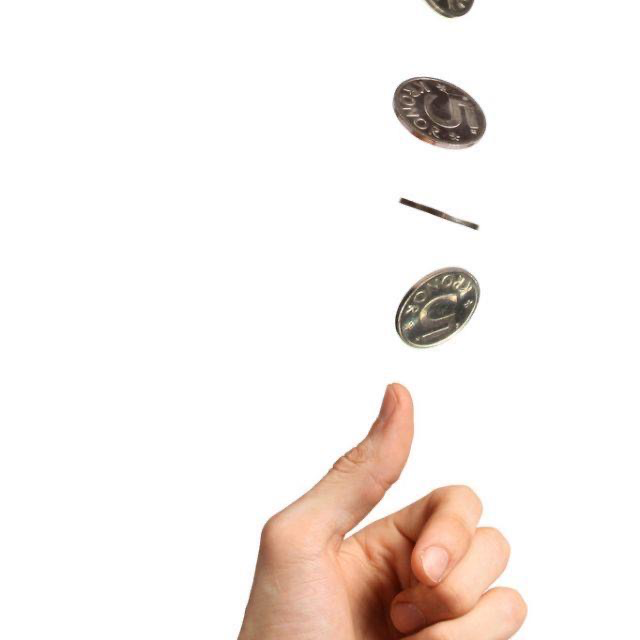
\includegraphics[width=0.5\linewidth]{asset/20230915222104.png}
  \caption{}
  \label{fig:img20_1}
\end{figure}

原因在于, 你不管抛多少次, 正反面出现的次数相互之间不会有太大的差异. 比如, 我不可能抛100次硬币99次正面朝上, 1次反面朝上, 这种情况发生的几率非常非常小. 

所以我们在遇到一些决定不了的事情, 尤其是古人, 他们有一些神灵崇拜的东西, 他们就觉得选择抛一些硬币, 哪一面朝上就代表了上天的意愿, 我们就要遵守上天的意愿. 

当然, 在现代的一个科学时代, 从科学的角度去解释应该怎么样去理解它?通过大量的一个实验, 我们会发现正反面出现的这个频率是趋于相同的, 就比如说在100次当中正面可能出现47次, 反面出现53次. 他们出现的频率, 基本上相差不多, 都是在0.5左右. 而在这里就有两个概念, 一个是频数, 一个是频率. 

它们代表的是什么意思呢?频数代表了变量值中某一个特征的数出现的次数. 比如, 在我们抛硬币的这个例子里, 可以说正面朝上出现的频数是多少, 那正面朝上在这里就代表了一个特征. 频率就是这个特征对应的这个频数与你总共进行的实验次数之比. 

\section{频率派视角下的概率}

在概率的世界里面有一个派别叫做频率派, 我们现在对于概率的定义主要还是采用了频率派的思想. 

在频率派中对概率的定义为: 当我们做大量的重复实验的时候, 随着这个实验次数的增加, 某一个事件出生的一频率, 总是在一个定值的附近稳定的摆动, 我们就把这个定值称为这个事件发生的概率. 

所以你看, 通过频率派的这个概率定义我们可以发现一个事件的概率是通过做大量重复试验所得出的那个频率来进行预估的. 那好了, 在生活当中有哪一些比较有趣的例子是用到了这种概念?

比如, 在足球比赛的时候一开始裁判就会把两队的队长叫到一起, 然后抛硬币来挑边, 决定谁先开球谁挑边. 而这个也是因为按照频率派的定义, 正反面朝上的频率是一样的. 

还有包括在赌场有一些游戏是掷骰子猜大小, 1、2、3点为小, 4、5、6点为大. 那为什么很多人在赌场会玩这种游戏呢?就是因为客观理性的来说, 如果不对骰子去做什么手脚的话, 那1、2、3点出现的频率和4、5、6点, 所对应的基本事件出现的频率是相等的. 

\begin{figure}[ht]
  \centering
  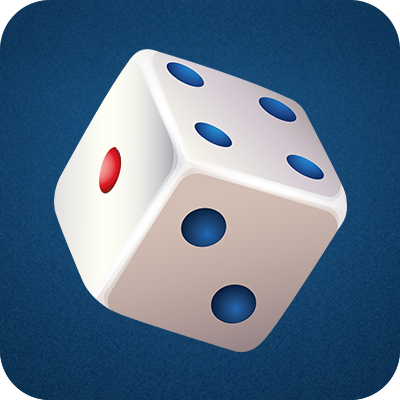
\includegraphics[width=0.3\linewidth]{asset/20230916012942.png}
  \caption{}
  \label{fig:img20_2}
\end{figure}

然后还有一个例子, 我记得有个故事是这么说的: 在古代有一个将军, 他本来要带领他的队伍上前线去抗击敌人, 但是这个时候部队的士气非常的低迷, 因为他们已经打了很多场败仗了. 所以这个时候将军就想到一个点子, 抓了一大把铜钱, 然后把所有的将士都召集在一起, 当着所有将士的面说, 我现在就在这里把这么多的铜钱全部当着你们的面给抛出去, 如果所有的铜钱都是正面朝上的话就说明是天神护佑我们, 我们这场仗就一定能赢. 他把这把铜钱全部撒出去的时候还真的就是所有铜钱都是正面朝上, 士兵一下子受到了鼓舞, 因为他们信以为真了, 觉得这个真的是天神的意愿. 

按照我们现代科学的角度来理解, 如果是正常的这个铜钱的话我们不能说铜钱所有面都朝上的概率为0, 但是我们每个人都清楚, 发生的概率微乎其微, 所以那些将士也没有怀疑这个将军会骗他们. 但是其实, 这个铜钱是做了手脚的, 两面其实都是正面. 士兵们没想到这个, 所以他们就想, 这么小概率的事情都能发生, 那真的是天神来护佑. 所以, 古代人其实对于频率的了解已经比我们想象的要深入的多了. 

在这个频率派视角下的概率还有一些比较有意思的一些科学案例, 其中一个就是这个布丰投针试验: 简单来说, 就是我们弄一张白纸, 然后这些纸上面会有一些平行线. 比如说这些线之间是有一个间距的, 其间距为t. 然后我们也准备了一大把的针, 这些针的长度为l, 并且, l小于平行线之间间距, 也就是l<t. 然后我们就往这个纸上面投针. 

\begin{figure}[ht]
  \centering
  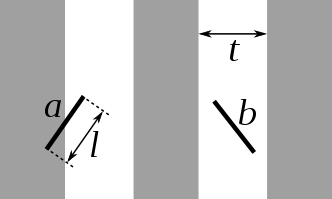
\includegraphics[width=0.6\linewidth]{asset/20230916012927.png}
  \caption{}
  \label{fig:img20_3}
\end{figure}

说到这里, 我们为什么要这么做呢?为什么我们要准备一张纸然后画这些平行线, 准备这种长度的针往这个纸上面投呢?因为我们想通过这个方式去计算圆周率, 这个听上去是不是觉得有点不可思议?在这个图上面完全看不到任何跟圆相关的东西, 只是一些平行线, 然后有两根针在这里, 就通过简简单单的撒针我们就可以找出这个圆周率吗?

其实是真的可以找出来, 这就是一个比较神奇的事情. 现在, 我们先把实验放一边, 先从理论进行分析, 判断这个针和这些平行线相交的概率会有多少?而这个概率里面会包含着一个圆周率派. 

当我们往这个纸上面投针的时候, 比如说我们往这个纸上面投针n次, 然后我们把针和直线相交的这些次数记为m. 用两个随机变量$X$和$Y$, $X$用来表示针的中点到最近的平行线的距离, $Y$表示针与平行线的夹角. 

如何用$X, Y$来表示这个针与直线是否相交呢?当针与直线相交的时候, 必定$X < l/2$, 然后乘上$sinY$. 也就是$X < l / 2sinY$. 

并且$X$在$(0, t/2)$内服从均匀分布, $Y$在$(0, \pi/2)$内服从均匀分布, $X, Y$相互独立. 也就是说, $t/2$这个位置的任何一处, 机会都是均等的, 不存在哪个地方出现的概率大, 哪个地方出现的概率小这种问题, $Y$也是如此. 

则$X, Y$的概率密度函数为: 

\begin{align*}
  f(x,y) &  = \begin{cases} 
  \frac{4}{\pi t} \\ 0 
  \end{cases} 
  0 < x < \frac{t}{2}, 0 < y < \frac{\pi}{2} \\
  P(\mbox{针与直线相交}) &  = P(X < \frac{l}{2}sinY) \\
  & = \int_0^{\frac{\pi}{2}} \int_0^{\frac{l}{2}siny}\frac{4}{\pi t}dxdy 
  \quad = \frac{2l}{\pi t}
\end{align*}

我们对这个概率密度函数取积分, 积分对应的面积就是概率. 

在之前我们在讲运动学那个例子的时候, 也就是讲解导数的时候曾经说过位移和速度那两个函数图像. 在那个位移图像, 两个点的纵坐标之差, 就是位移的差, 或者说这个点移动了多少位移. 在速度图像上面是两个点和函数曲线以及这个x轴所围成的面积, 形成了这个点移动的面积. 

概率密度函数就和速度图像很像, 它和坐标轴以及两个点围成的这个面积构成的某一块的这个概率代表了概率的大小. 

所以在这里我们会发现在$x$和$y$各自的定义域里面, $x$在$(0, t/2)$是均匀分布的, 那它加在一起的概率就为1. 那拿1除以这个区间的长度, 就是这个区间的概率密度. 1除以$t/2$就得到$2/t$. 同理我们拿1去除这个区间的长度$\pi /2$也就是$2/\pi$, 就对应的y在这个区间内的概率密度. 整个区间乘上它的概率密度, 就等于它们的概率为1. 因为y只在这里分布, 其他地方没有分布. 

它们两个因为是相互独立的, 所以他们的概率密度可以直接相乘, 得到两个量联合的一个概率密度函数. 在他们定义域之外, 比如$X < 0$的时候, 那他们出现的概率都是0. 

接下来我们来看一下这个针与直线相交概率对应的这个式子对不对. 这个式子包含的数学意义可以通过双重积分来代表. 双重积分并不难, 双重积分其实就相当于做两次积分, 先积里面这一层, 里面这一层积出来之后再积外面这一层. 这个看上去很唬人很复杂, 其实就是那么回事. 

我们先来对$X$去进行积分,然后再对$Y$去进行积分. 求出来之后, 我们说过概率密度是面积对应着概率, 所以这个积分干的就是求面积的事. 根据微积分那一节课里面所上到的内容, 大家可以求出来这个值呢是$2l/\pi t$. 

到此为止这个理论分析了就结束了, 为什么我们在这里需要进行这个理论分析呢?因为当我们通过理论分析把这个事件发生的这个概率求出来之后, 我们就能发现里面有个$\pi$, 有个$\pi$有什么惊奇的?接下来第二点就来了. 

按照频率派的这个原则, 我们可以用频率去估计概率, 只要我进行大量投针实验, 统计一下针与直线相交事件出现的这个频率, 我们就可以用这个频率来当做它的概率, 也就是说现在都是一些已知量, 唯一的未知量就是派. 所以根据这个我们就可以通过做大量的投针实验把派给计算出来. 

其实, 这一现象也并不难理解, 主要是对应着两点, 一个是在地球自转效应, 一个是引力场效应. 它揭示了地球自转和引力对物体运动的影响. 这一实验也成为了地球物理学和力学研究的一个重要示例, 用来解释自然界中的现象. 布丰投针试验的成功也帮助加强了牛顿引力定律的理论基础, 这对于现代科学的发展具有重要意义. 

所以你看, 这个投针实验和$\pi$看似完全没有任何关系, 但是结果我们发现真的就通过简简单单的投针, 就能把这个圆周率派给求出来. 不需要通过非常严密的数值计算、数值分析方面的一些处理, 就简单的去投针就行了. 

当然, 这个投针实验是一个比较理想化的一个模型, 因为这个频率有的时候不是很稳定, 所以导致估算出来这个概率也往往不是特别准确, 导致计算出来这个$\pi$值往往不一定是比较好的一个解. 比如只能精确到小数点后两位, 再往下进行就不行了. 但是这并不妨碍我们通过这么一个视角来了解一下原来大自然是很神奇的, 各个量之间其实都是有一些联系的, 而不是彼此独立的. 

我们现在再来全面的看一下, 频率派看待这个概率有哪一些性质呢?

首先, 因为是通过频率来估算概率的, 所以实验必须是可以进行很多次, 而且要易于操作, 成本也低, 周期也要短. 不能做一个实验花十天半个月的, 那你别说做1,000次了, 十次都够呛. 

第二个, 缺乏一定的严谨性, 这个就是我刚才说的, 因为通过频率去估算概率的话, 这个和你实际上去做这些实验的结果有非常大的关系. 而这个实验结果可能会受到各种各样意想不到的一些因素的干扰. 各种错综复杂的小细节都会影响到最终结果. 所以, 往往会导致你这个频率本身就不太稳定. 

第三, 无法对不可多次重复的事件去进行预判. 比如去做一些药物的毒理性检测的时候, 或者说去测量某种生物的一个抗毒性的时候, 你不可能像投针、投硬币那样. 也许有更好的一种方式去分析, 所以在这种情况下, 频率派呢就没法去处理了. 

第四, 频率派天然的觉得事件本身就是随机的, 不是我们能力不够, 不是我们人类太low, 是因为大自然本身很多事情就是随机的, 这是客观规律. 然后另外一个流派跳出来了: 贝叶斯派. 

\section{贝叶斯派视角下的概率}

他一上来就直接和频率派掐架, 频率派说, 客观世界是内在的存在一些随机性, 这个是自然规律, 是普遍存在的. 然后贝叶斯派说不, 并没有这个什么客观的随机性, 只是因为我们人类作为一个观察者没有上帝视角. 

频率派说我们要找出正确的概率模型参数, 它是客观存在且唯一正确的. 就是我们对于一个概率模型它是有一些参数的. 一种概率模型它有哪些参数呢?有均值、方差, 这些都可以算作是一个概率模型的参数. 

那往往概率的框架定下来之后, 我们把概率的参数确定了之后, 这个模型就掌握了. 我们就可以说我们已经找到了正确的概率模型了. 频率派就认为这样的参数是客观存在而且是唯一正确的. 

当然贝耶斯派又不同意了, 他说我们都没有上帝视角, 你咋那么确信你找出来那一个就是正确的呢?你咋就知道其他的就一定不是正确的呢?

所以对于贝叶斯派而言, 他们认为这个所谓的随机只是由于人类没有办法掌握全局信息. 什么叫做人没有办法掌握全局信息呢?

比如, 很多同学玩Dota或者其他什么游戏, 当你在那个地图上面的时候你这个人物角色是能看到全地图的吗?你是不能的对吧, 只能掌握到某一个范围之内. 你这个人物活动范围之内的一个信息, 而超过这个范围之外的那些
信息你是不知道的. 所以人也是一样, 没有办法掌握全局信息, 超过我们认知范围之外的那些东西我们都不掌握. 

所以对于这些有内幕消息的人来说, 股市的波动他是确定的, 因为有小道消息他知道哪一个股会上涨或者说下跌. 但是对于普通散户来说, 就没有这么多的信息来源, 所以就是两眼一抓瞎, 就觉得股市的波动是随机的, 是不确定. 

所以贝叶斯派把这个概率视为对某种结果出现的一个信任的程度, 而不是频率. 就比如说他对一个事件的两种结果a和b, 贝耶斯派给出了$a$概率为$0.6$、$b$概率为$0.4$, 不是说$a$出现的这个频率是$0.6$, $b$出现频率是$0.4$. 贝叶斯派是认为我们有$60\%$的信心相信$a$会出现, 而我们同样有$40\%$的信心认为$b$会发生. 贝叶斯是这样理解的. 

